\subsubsection{Acopladores ópticos}

% SLIDE DE ACOPLADORES ÓPTICOS
\begin{frame}
\frametitle{Acopladores ópticos}

Os acopladores ópticos são dispositivos que operam por meio de um feixe de luz, 
para transmitir sinais de um circuito para outro.
O led emite um sinal infra vermelho, o foto transistor capta e satura,
conduzindo corrente do coletor para o emissor.

\begin{figure}
\centering
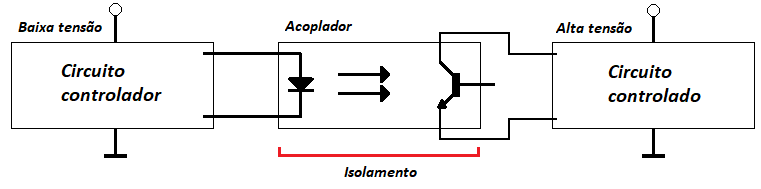
\includegraphics[scale = 0.4]{figuras/acoplador}
\end{figure}

\begin{figure}
\centering
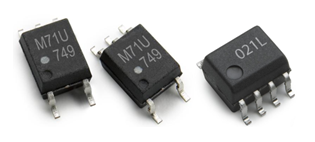
\includegraphics[scale = 0.2]{figuras/fotoacoplador}
\end{figure}

\end{frame}
